%! TEX root = ../../master.tex
\lecture[Simplices. $\Delta$-complexes. Torus, Klein Bottle, $\mathbb{R}\mathbb{P}^2$ and $S^n$ as  $\Delta$-complexes. Chains, chain complexes. Homology groups. Homology groups of $S^1$]{Mi 13 Okt 2021}{$\Delta$-complexes}

\begin{orga}
    \begin{itemize}
    \item All lectures will be recorded and uploaded to eCampus afterwards.
    \item The same holds for all written lecture notes (from the iPad).
    \item Daniel is happy if you turn on your camera, these will not be recorded
    \item If you have questions, feel free to ask them at any time. Beware that your voice / question will be recorded
    \item It is not yet know whether the exam at the end of the semester will be in person or online.
    \item You can also ask questions in the chat (these will not be recorded) if you prefer so.
    \item There is an question session on Monday, 10. You can ask questions there, but there will also be questions asked to the students that are to be solved 'live'.
    \item On next Monday, we will quickly summarize the basics of category theory
    \item You need 50\% of the points obtainable from the exercise sheet to be admissible to the exam.
    \item For everything taking place at the university (question session or exercise groups) you are required to fulfill the 3G rule: be vaccinated against, recovered from or testet for the coronavirus.
    \item If you did not attend the course on 'Geometrie und Topologie' the last semester, you can have a look at the lecture notes \cite{geotopo}. These are in German, though. You can also visit the corresponding \href{https://ecampus.uni-bonn.de/goto_ecampus_crs_2122054.html}{eCampus course} or the \href{http://www.math.uni-bonn.de/people/daniel/2021/geotopo/}{webpage}.
    \item If you want to write a bachelor thesis in topology, during one of the lecture times in January, all the topology group members will be present and present a number of topics for a Bachelor thesis. So don't ask yet for possible topics.
    \item Exercise sheets can be handed in groups of up to 3 people. Everyone is required to understand all the solutions
    \end{itemize}
\end{orga}

As literature, \cite{algebraische-topologie-lueck} (in german) and \cite{algebraic-topology-hatcher} are recommended.

\setcounter{section}{-1}
\section{Motivation for this lecture}

Last semester we had a look at
\begin{itemize}
    \item basic properties of topological spaces (e.g. Hausdorff or compact spaces)
    \item The fundamental group of a topological space, coverings to compute it
    \item Fundamental results we proved were:
        \[
            \pi_1(S^1,1)\cong \mathbb{Z} \qquad \pi_1(S^n, s_0) = 0 \qquad \forall n\geq 2
        \] 
\end{itemize}

We aim to kind of generalize this to higher n, one can in fact define
\[
    \pi_n(X,x_0) = [(S^n,s_0), (X,x_0)]
\] 
but these are very hard to compute and do not behave as one would possibly expect from a generalization, e.g. it holds
\[
    \pi_3(S^2,s_0) \cong \mathbb{Z}
\] 
We will consider \vocab{homology} instead. Homology is much harder to define than the higher homotopy groups, but will be much easier to compute.

\begin{warning}
    We will consider $R$-modules in this course. If you are not familiar with them, just tell Daniel or ask questions at any time.
\end{warning}

For now, just think of modules as a sort of vector space, but over a ring $R$, not a field  $K$.

At the start we will only consider $\mathbb{Z}$-modules, i.e. abelian groups.


\section{$\Delta$-complexes \& semi-simplicial sets}
\subsection{$\Delta$-complexes}

\begin{definition}[simplex]\label{def:simplex}
    The \vocab{$n$-simplex} is the space
    \[
        \Delta^n = \left \{(t_0,\ldots,t_n)\in \mathbb{R}^{n+1} \mid  \sum_{i=0}^n t_i = 1, t_i \geq  0\right\} 
    \]
    That is, $\Delta^n$ is the convex subspace of  $\mathbb{R}^{n+1}$ spanned by
    \[
        e_0 =(1,0,\ldots,0), \ldots, e_n = (0,0,\ldots,1)
    \] 
\end{definition}


\begin{example}[low dimensional simplices]\label{ex:small-simplices}
    Have a look at \autoref{fig:simplices}:
\item $\Delta^0$ is just a point.
\item  $\Delta^1$ is the unit interval via the embedding
        \begin{equation*}
        \begin{array}{c c l} 
            \left[0,1\right] & \longrightarrow & \mathbb{R}^2 \\
            t & \longmapsto &  te_0 + (1-t)e_1
        \end{array}
    \end{equation*}
\item $\Delta^2$ is a triangle
\item $\Delta^3$ is a tetrahedron
\end{example}

\begin{figure}
    \centering
    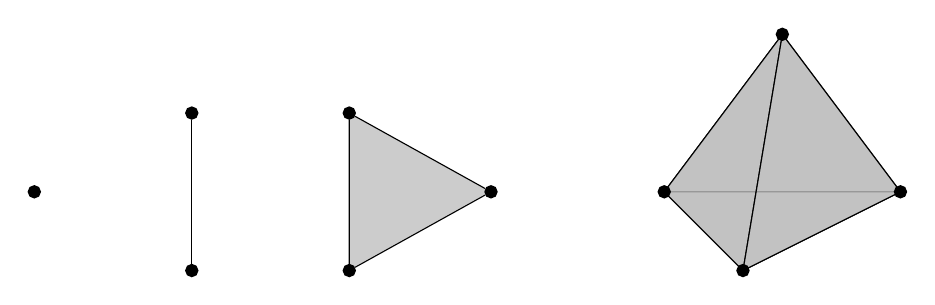
\begin{tikzpicture}
            \tikzstyle{point}=[circle,thick,draw=black,fill=black,inner sep=0pt,minimum width=4pt,minimum height=4pt]
            \tikzstyle{simplexfill} = [fill = Gray!50!White, fill opacity = 0.8]
            \node (a)[point] at (-6,0) {};
            \node (b1)[point] at (-4,-1) {};
            \node (b2)[point] at (-4,1) {};
            \draw (b1) -- (b2);
            \fill[simplexfill] (-2,-1) -- (-2,1) -- (-0.2,0) -- cycle;
            \node (c1)[point] at (-2,-1) {};
            \node (c2)[point] at (-2,1) {};
            \node (c3)[point] at (-0.2,0) {};
            \draw (c1) -- (c2) -- (c3) -- (c1);

            \coordinate (d1) at (2,0);
            \coordinate (d2) at (3,-1);
            \coordinate (d3) at (5,0);
            \coordinate (d4) at (3.5,2);
            \draw[simplexfill] (d1) -- (d3) -- (d4) -- cycle;
            \draw[simplexfill] (d1) -- (d2) -- (d3) -- cycle;
            \draw[simplexfill] (d1) -- (d2) -- (d4) -- cycle;
            \draw[simplexfill] (d2) -- (d3) -- (d4) -- cycle;
            \node[point] at (d1) {};
            \node[point] at (d2) {};
            \node[point] at (d3) {};
            \node[point] at (d4) {};
    \end{tikzpicture}
    \caption{some first simplices}
    \label{fig:simplices}
\end{figure}

\begin{definition}[face]\label{def:face}
    For a subset $I\subset \left \{0,\ldots,n\right\} $ consider the subspace
    \[
        \left \{(t_0,\ldots,t_n) \in \Delta^n \mid  t_i = 0 \; \forall i \in I\right\} 
    \] 
    This is called a \vocab{face} of or also $(n-\abs{I} )$-face of $\Delta^n$.

\end{definition}


\begin{definition*}[inclusion]\label{def:inclusion}
    For $0\leq i\leq n$ define
        \begin{equation*}
        \delta^i = \delta^{n,i}: \left| \begin{array}{c c l} 
        \Delta^{n-1} & \longrightarrow & \Delta^n \\
        (t_0,\ldots,t_{n-1}) & \longmapsto &  (t_0,\ldots,t_{i-1},0,t_i,\ldots,t_{n-1})
        \end{array} \right.
    \end{equation*}

    $\delta^i$ is the \vocab{inclusion} of the $i$th face of  $\Delta^n$
\end{definition*}

\begin{definition*}[boundary]\label{def:boundary}
The \vocab{boundary} $\partial\Delta^n$ of $\Delta^n$ is the union of the highest dimensional faces, i.e.
     \[
         \partial\Delta^n \coloneqq  \bigcup_{i=0} ^n \im δ^i = \left \{(t_0,\ldots,t_n) \in \Delta^n \mid  \exists i\colon  t_i = 0\right\} 
    \] 
    
\end{definition*}

\begin{definition*}[interior]\label{def:interior}
The \vocab{interior} of $\Delta^n$ is defined as
    \[
        \mathring{\Delta}^n \coloneqq  \Delta^n \setminus \partial\Delta^n
    \] 
    
\end{definition*}

\begin{remark**}
    Note that the boundary of the 0-simplex is empty, since there are no $-1$-dimensional faces of the 0-simplex. This also means that  $\mathring{\Delta}^0 = \Delta^0$.
\end{remark**}

\begin{definition}[$\Delta$-complex]\label{def:delta-complex}
    A  \vocab{$\Delta$-complex} is a topological space $X$ together with the following structure:

    For all $n\in \mathbb{N}_0$, there is a set $A_n = \left \{α\colon  \Delta^n \to  X\right\} $ such that
    \begin{enumerate}[1)]
        \item $\forall α\in A_n$, the restriction $α\mid _{\mathring{\Delta}^n}$ is injective
        \item $\forall x\in X$, there is a unique pair  $(n,α)$ with  $n\in \mathbb{N}_0$ and $α\in A_n$ such that $x\in α\mid _{\mathring{\Delta}^n}$ 
        \item $\forall α\in \Delta^n$ and $i\in \left \{0,\ldots,n\right\}$ we have $α \circ  \delta^i \in  A_{n-1}$.
        \item A subset $U\subset X$ is open iff
            \[
                α^{-1}(U) \subset \Delta^n \text{ is open } \forall n\in \mathbb{N}_0, α\in A_n
            \] 
    \end{enumerate}
\end{definition}


\begin{oral}
    The last property essentially tells us that you can recover the topology on $X$ from the sets of maps $A_n$.

    Beware that the set of maps $A_n$ is not necessarily the set of all maps, this set is part of the data of the $\Delta$-complex.
\end{oral}

\begin{placeholder}
    In the lecture, 1.5 was somehow skipped.
\end{placeholder}

\begin{example}[Torus as $\Delta$-complex]\label{ex:delta-complex-torus}
    Considering the torus as a quotient from $I^2$ (the unit square).

    \missingfigure{Torus as a $\Delta$-complex}

    Inserting a diagonal into the unit square realizes the torus as a $\Delta$-complex with two 2-simplices (namely the two triangles), three 1-simplices (the diagonal, and the two pairs of opposite sides of the square) and one 0-simplex (the corners of the square that are glued together)

    Note that in this case $A_n = \emptyset$ for $n\geq 3$.
\end{example}

\begin{example*}[Klein bottle as $\Delta$-complex]\label{ex:klein-bottle-delta-complex}
    We can also realize the \vocab{Klein bottle} as a simplicial complex, just as we did with the torus
    \missingfigure{klein bottle as $\Delta$-complex}
\end{example*}

\begin{example*}[$\mathbb{R}\mathbb{P}^2$ as simplicial complex]\label{ex:delta-complex-projective-space}
    We can do the same for $\mathbb{R}\mathbb{P}^2$.
    \missingfigure{$\mathbb{R}\mathbb{P}^2$} 
\end{example*}

\begin{example*}[$S^n$ as simplicial complex]\label{ex:delta-complex-sphere}
    For $S^n$ (the unit sphere), there are a lot of examples:

    \missingfigure{Sphere} 
   
    We can also consider $S^1$ as  $\faktor{\Delta^1}{\partial\Delta^1}$ as a $\Delta$-complex, but this won't hold for $n\geq 2$, since the embeddings of the interiors of the maps won't be injective anymore, so they don't satisfy the requirements of a structure.
\end{example*}

\begin{remark}\label{rm:ordered-simplicial-complex}
    \begin{itemize}
        \item 
    There is also the notion of (an ordered) simplicial complex.  This is slightly more restrictive: We assume that for $α,β\in A_n$ it follows $α = β$ if 
     \[
    α \circ  δ^i = β \circ  δ^i \qquad \forall  i=0,\ldots,n
    \] 
    i.e. if they have the same $0$-faces.

    \missingfigure{Triangle and circle}
\item A $\Delta$-complex can be turned into a simplicial complex by  \vocab{centric subdivision}:

    \missingfigure{centric subdivision}
    We will not define this for now.
    \end{itemize}
\end{remark}


\subsection{Simplicial homology}

\begin{definition}[chains, boudary homomorphism]\label{def:chains-boundary-homomorphism}
   Let $X$ be a  $\Delta$-complex.
   \begin{itemize}
       \item The  \vocab{$n$-chains} of $X$ are the free abelian groups  $\Delta_n(X)$ generated by $A_n$, i.e.
           \[
               \Delta_n(X) \coloneqq  \mathbb{Z}\left[ A_n \right] \cong \bigoplus_{A_n} \mathbb{Z}
           \] 
       \item The \vocab{boundary homomorphism} is defined as
               \begin{equation*}
               \partial_n: \left| \begin{array}{c c l} 
                   \Delta_n(X) & \longrightarrow & \Delta_{n-1}(X) \\
                   α & \longmapsto &  \sum\limits_{i=0}^{n}(-1)^i(α \circ  δ^i)
               \end{array} \right.
           \end{equation*}
   \end{itemize}
\end{definition}

\begin{lemma}\label{lm:composition-of-boundary-maps-index-swapping}
    If $i\leq j$, then 
    \[
        δ^i \circ  δ^j = δ^{j+1} \circ δ^i\colon \Delta^{n-2} \to \Delta^n 
    \]
\end{lemma}

\begin{proof}
    We have
    \[
        (t_0,\ldots,t_{n-2}) \stackrel{δ^j}{\longrightarrow} (t_0,\ldots,t_{j-1},0,\ldots,t_j,\ldots,t_{n-2}) \stackrel{δ^i}{\longrightarrow} (t_0,\ldots,t_{i-1},0,t_i,\ldots,t_{j-1},0,t_{j},\ldots,t_{n-2})
    \] 
    Note that if $i=j$,  $t_i,\ldots,t_{j-1}$ expands to nothing, i.e. the two zeros will be adjacent to each other. For the other composition, we have
    \[
        (t_0,\ldots, t_{n-2}) \stackrel{δ^i}{\longrightarrow} (t_0,\ldots,t_{i-1},0,t_i,\ldots,t_{n-2}) \stackrel{δ^{j+1}}{\longrightarrow} (t_0,\ldots,t_{i-1},0,t_i,\ldots,t_{j-1},0,t_j,\ldots,t_{n-2})
    \] 
    Also for $j=i$ we have the zeros being adjacent.

    Now we directly see that these are in fact the same maps.
\end{proof}

\begin{lemma}\label{lm:composition-of-boundaries-is-zero}
   It holds $\partial_{n-1} \circ  \partial_n = 0$. 
\end{lemma}

\begin{proof}
   We compute the composition:
   \begin{IEEEeqnarray*}{rCl}
       \partial_{n-1}(\partial_n(α)) & = & \sum_{j=0}^{n-1}\sum_{i=0}^n (-1)^{i+j}(α \circ  δ^i \circ  δ^j) \\
                                     & = & \sum_{j=0}^{n-1} \sum_{i=0}^j (-1)^{i+j}(α \circ  δ^i \circ  δ^j) + \sum_{j=0}^{n-1}\sum_{i=j+1}^n (-1)^{i+j}(α\circ δ^i \circ δ^j) \\
                                     & \stackrel{\autoref{lm:composition-of-boundary-maps-index-swapping}}{=}  & \sum_{j=0}^{n-1} \sum_{i=0}^{j}(-1)^{i+j}(α \circ δ^{j+1} \circ δ^i) + \sum_{i=1}^{n} \sum_{j=0}^{i-1} (-1)^{i+j}(α \circ δ^i \circ δ^j) \\
                                     & = & \sum_{j=0}^{n-1} \sum_{i=0}^{j} (-1)^{i+j} (α \circ  δ^{j+1} \circ  δ^i) + \sum_{i=0}^{n-1} \sum_{j=0}^{i} (-1)^{i+j+1} (α \circ  δ^{i+1} \circ  δ^j) \\
                                     & = & 0
   \end{IEEEeqnarray*}
\end{proof}

\begin{definition}[chain complex]\label{def:chain-complex}
    A \vocab{chain complex} $(C_{\chainbullet }, \partial_{\chainbullet })$ of $\mathbb{Z}$-modules is a sequence of abelian groups:
    \[
    \ldots \to C_n \stackrel{\partial_n}{\longrightarrow} C_{n-1}\stackrel{\partial_{n-1}}{\longrightarrow} C_{n-2}\to \ldots\to C_1 \stackrel{\partial_1}{\longrightarrow} C_0 \stackrel{\partial_0}{\longrightarrow} 0
    \] 
    such that $\partial_{n-1}\circ \partial_n = 0$ for all $n\geq 1$.

    The chain complex is called \vocab{exact} if $\ker \partial_n = \im \partial_{n+1}$  for all $n$.
\end{definition}

\begin{remark*}
    Note that the condition $\partial_{n-1} \circ  \partial_n = 0$ just imposes the condition $\im \partial_{n+1} \subset \ker \partial_n$
\end{remark*}

\begin{example}\label{ex:homology-groups-are-delta-complex}
    Let $X$ be a  $\Delta$-complex. By \autoref{lm:composition-of-boundaries-is-zero}, $(\Delta_{\chainbullet }(X),\partial_{\chainbullet })$ is a chain complex.
\end{example}

\begin{definition}[homology group]\label{def:homology-group}
Let $(C_{\chainbullet},\partial_{\chainbullet })$ be a $\Delta$-complex. We define its \vocab{$n$-th homology group} by
    \[
    H_n(C_{\chainbullet} ,\partial_{\chainbullet }) \coloneqq  \faktor{\ker \partial_n}{\im \partial_{n+1}}
    \] 
\end{definition}

\begin{definition}
    Let $X$ be a  $\Delta$-complex. We define its \vocab{$n$th homology group} as 
    \[
        H_n^{\Delta} (X) = H_n(\Delta_{\chainbullet }(X),\partial_{\chainbullet })
    \] 
\end{definition}

\begin{example}
Pick $S^1$ as a $\Delta$-complex as in \autoref{ex:delta-complex-sphere}. Then $\Delta_0 \cong \Delta_1 \cong \mathbb{Z}$ and $\Delta_n = 0$ for $n\geq 2$. As $a \circ  δ^0 = a \circ  δ^1 = v$ we have
\[
    \partial_1(a) = a \circ  δ^0 - a \circ  δ^1 = v - v = 0
\] 
Thus the corresponding chain complex is:
\[
\ldots \to  0 \to  0 \to  0 \to  \mathbb{Z} \stackrel{0}{\longrightarrow} \mathbb{Z} \to  0
\] 
and thus
\[
    H_n^{\Delta}(S^1) \cong \begin{cases}
        \mathbb{Z} & n = 0,1 \\
        0 & n\geq 2
    \end{cases}
\] 
\end{example}
